The following sections are dedicated to the Camera Layer of this project. This layer includes Raspberry Pi Zero, database, stepper motor drivers, stepper motor, and camera module subsystems. The Camera Layer manages the actions set forth by the user in the Web Interface layer. The operating system used is Raspbian, while the programming language used is python. Besides the stepper motors components, a custom PCB board is used.

\subsection{Camera Layer}
The Raspberry Pi Zero will execute commands based on the user in the Web Interface layer. Once the user sets forth a command, the RPi Zero will execute and control the movements of the camera using the stepper motor driver to then control the stepper motors.

\subsection{Camera Layer Hardware}
Since the RPi zero has its own unique operating system, the operating system that will be used is Raspbian. 

\subsection{Camera Layer Software Dependencies}
Besides standard libraries that were installed, lwiringpi library had to be installed to allow functionality of the C++ code we were using at first to test the camera layer. Mjpeg will be used to as the video compressor since it would be the easier router for the amount of time to complete the project in the required time.The functionality is also dependent on the custom PCB stepper motor driver to control the stepper motors.


\subsection{Raspberry Pi Zero Subsystem}
Descibe at a high level the purpose and basic design of this subsystem. Is it a piece of hardware, a class, a web service, or something else? Note that each of the subsystem items below are meant to be specific to that subystem and not a repeat of anything discussed above for the overall layer.

\begin{figure}[h!]
	\centering
 	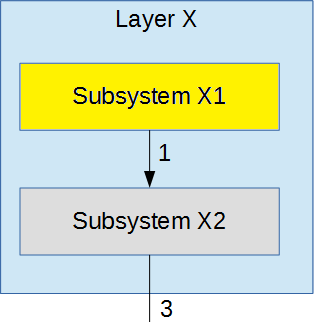
\includegraphics[width=0.60\textwidth]{images/subsystem}
 \caption{Example subsystem description diagram}
\end{figure}

\subsubsection{Subsystem Hardware}
A description of any involved hardware components for the subsystem.

\subsubsection{Subsystem Operating System}
A description of any operating systems required by the subsystem.

\subsubsection{Subsystem Software Dependencies}
A description of any software dependencies (libraries, frameworks, design software for mechanical parts or circuits, etc) required by the subsystem.

\subsubsection{Subsystem Programming Languages}
A description of any programming languages used by the subsystem.

\subsubsection{Subsystem Data Structures}
A description of any classes or other data structures that are worth discussing for the subsystem. For example, data being transmitted from a microcontroller to a PC via USB should be first be assembled into packets. What is the structure of the packets?

\subsubsection{Subsystem Data Processing}
A description of any algorithms or processing strategies that are worth discussing for the subsystem. If you are implementing a well-known algorithm, list it. If it is something unique to this project, discuss it in greater detail.


